\begin{sidewaysfigure}
	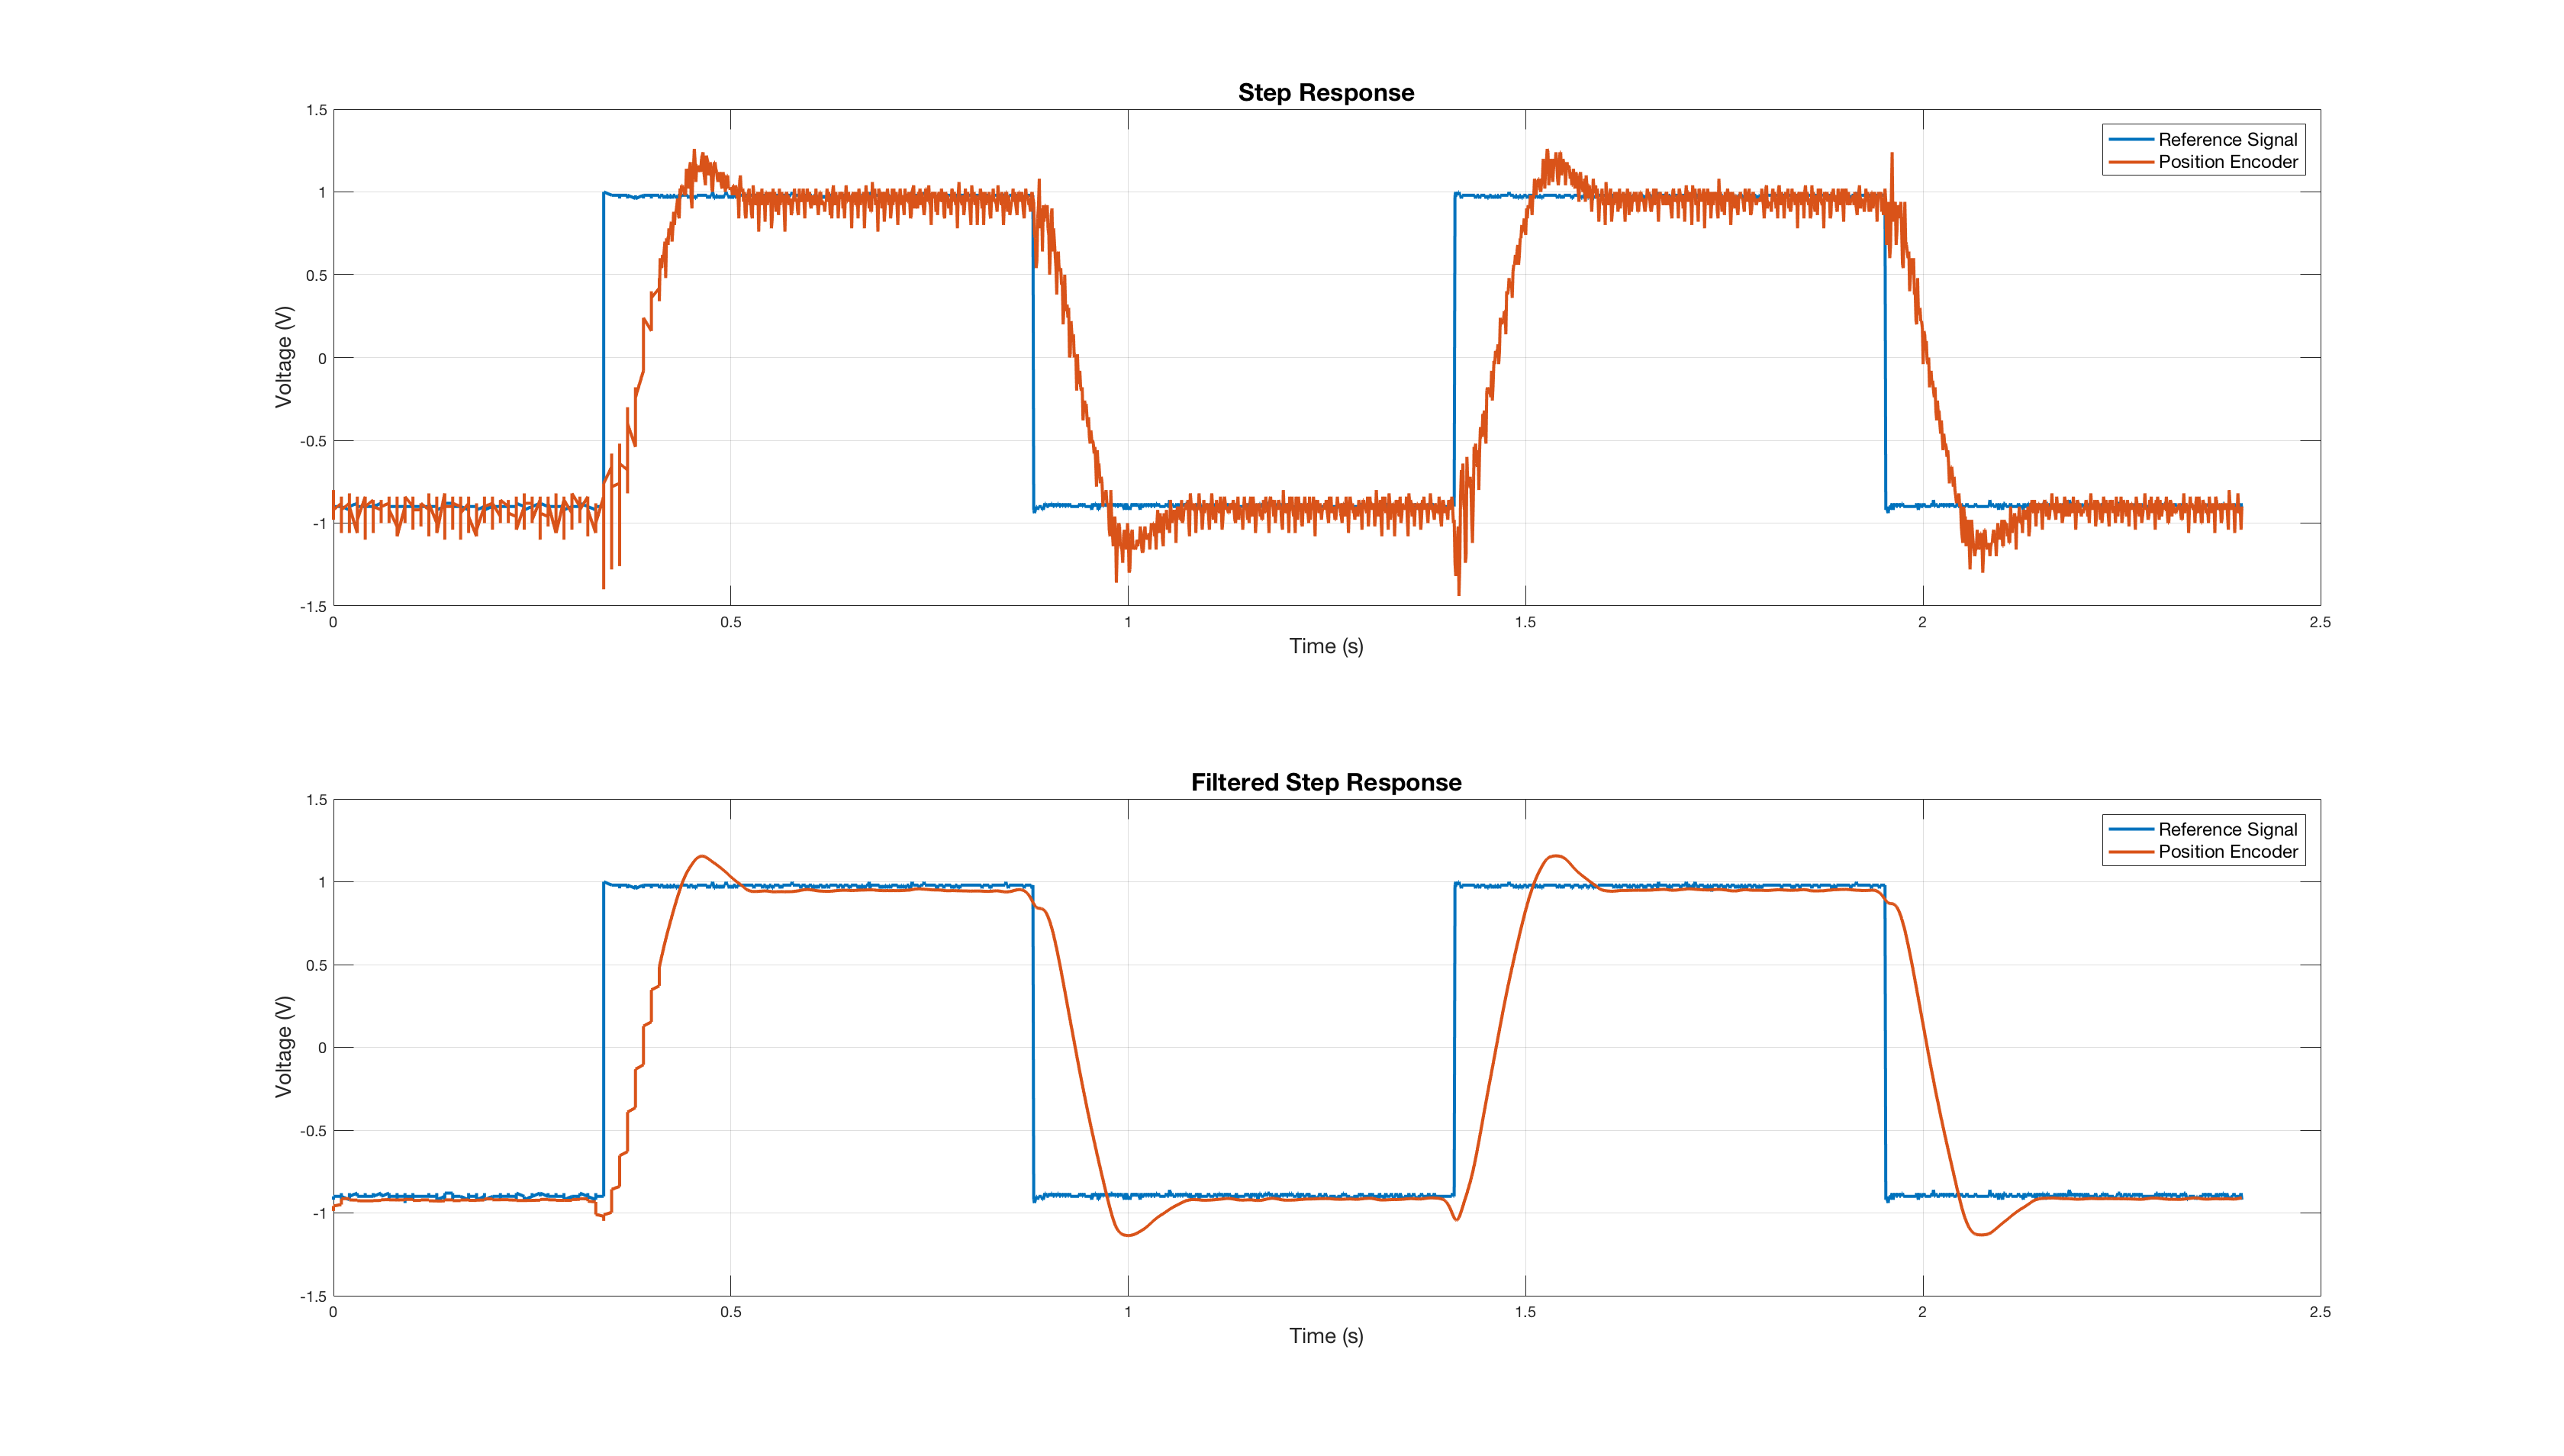
\includegraphics[width=\textheight]{img/results/step.png}
    \caption{Resposta do sistema à entrada degrau unitário. O sinal de referência foi gerado por um gerador de sinais, de amplitude $1V$ pico a pico e $1Hz$. Estão representados tanto o sinal original lido no osciloscópio, como um sinal filtrado para remover ruídos de alta frequência. Para a medição do erro em regime permanente, foi escolhido o ponto $time=0.8s$}
    \label{fig::step_response}
\end{sidewaysfigure}
